

Mining focuses on collecting ores by extracting them from rocks with a given pickaxe. The main modifiers to experience are the type of pickaxe and the type of ore. Mining success rates are actually much harder to find than woodcutting for example. As a result calculating experience rates is much more difficult. Instead, in this section we look at the \href{https://oldschool.runescape.wiki/w/Motherlode_Mine}{Motherload Mine} which is a very common mining technique. 

This activity enhances mining by providing a chance to obtain \emph{Gold Nuggets} which can be used to purchase rewards like the \emph{Prospector Outfit} that increases experience per ore mined. Each piece costs a certain amount, and each piece provides an experience boost, with more costly pieces providing more bonuses. So the natural question here is what order should the four pieces be purchased. With only four pieces a brute force approach is sufficient here as Fig.~\ref{fig:pay_dirt} reveals the optimal order to be 
\begin{equation}
\text{Jacket} \to \text{Legs} \to \text{Hat} \to \text{Boots},
\end{equation}
which is exactly the order of most expensive to least expensive items. The worst ordering is 
\begin{equation}
\text{Boots} \to \text{Hat} \to \text{Legs} \to \text{Jacket},
\end{equation}
which is the reverse of the optimal solution. Another way to visualize this is shown in Fig.~\ref{fig:mining_order}.


\begin{figure}
	\centering
	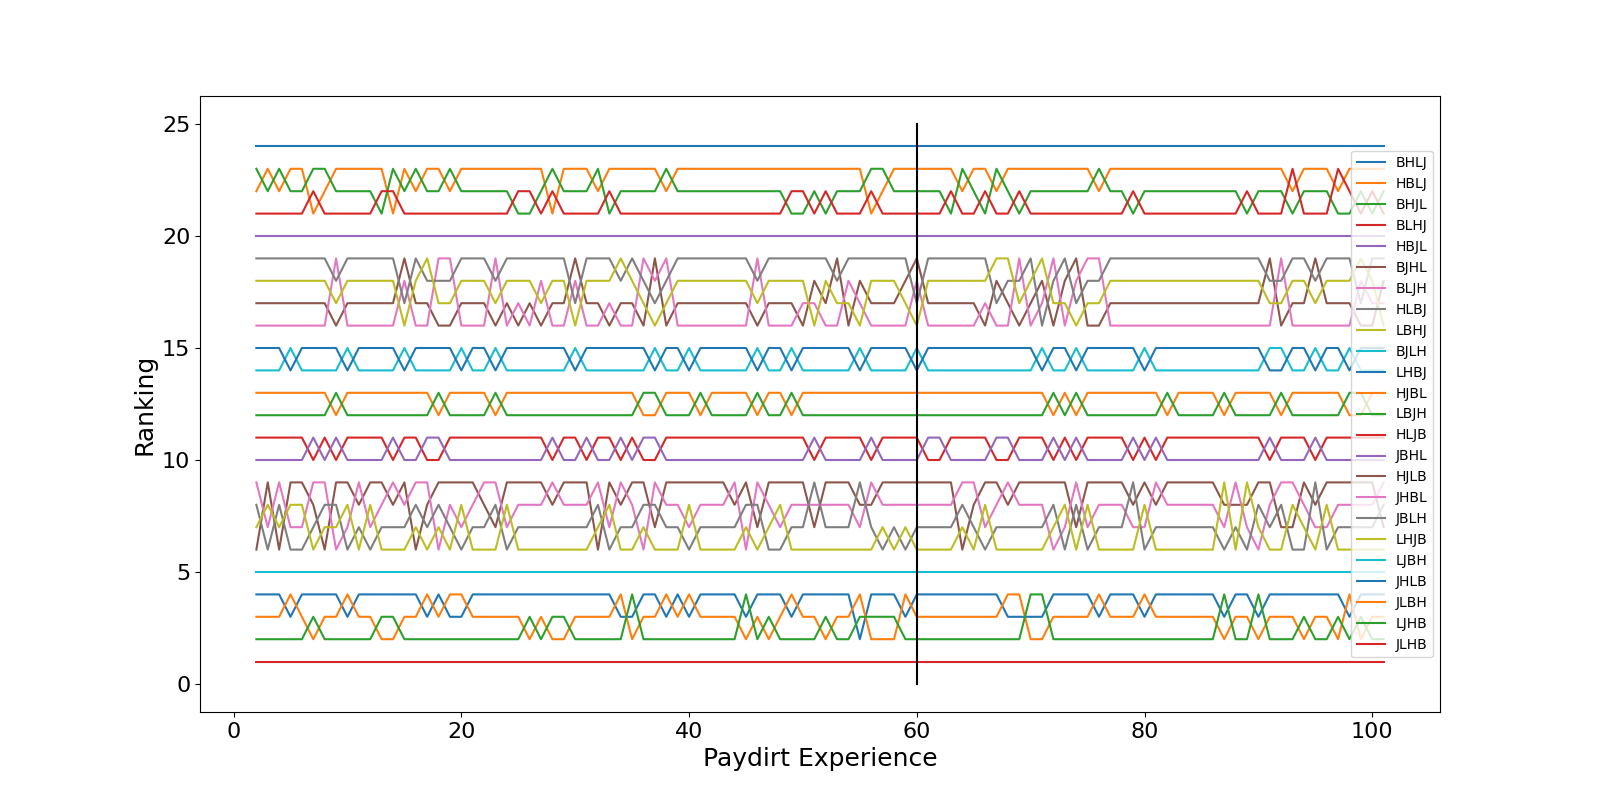
\includegraphics[width=\linewidth]{img/mining/varying_paydirt.100.png}
	\caption{
		A ranking of all possible orderings to obtain the full outfit. Notice that the x-axis here is the experience from the paydirt although this is fixed in game at 60, varying this parameter reveals that the order is very stable (rankings only change by 1 or 2). The order "JLHB" is the optimal, which "BHLJ" is the worst as it is the reverse order.
	}
	\label{fig:pay_dirt}
\end{figure}

\begin{figure}
	\centering
	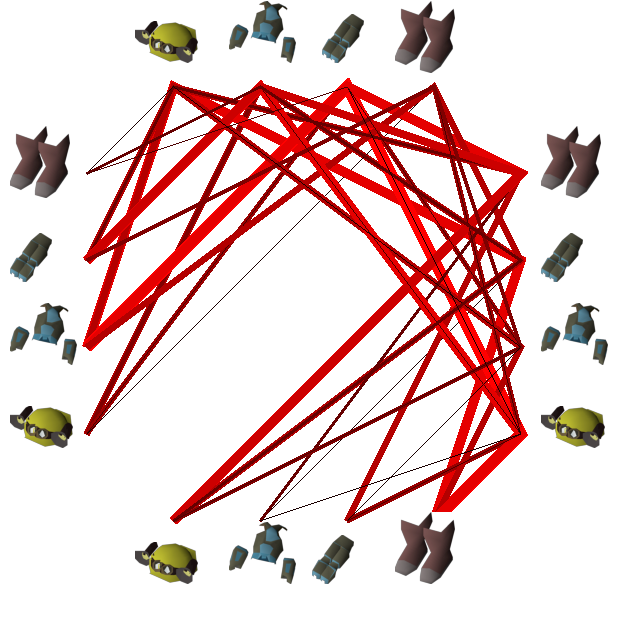
\includegraphics[width=0.5\linewidth]{img/mining/optimal_order.pdf}
	\caption{
		Starting on the left side, each line represents a possible ordering of obtaining the full set. The thickness of each line represents its rank. Clearly starting with the jacket (3rd row) is optimal, whereas starting with the boots (1st row) is worst. Said another way (looking at the bottom row), getting the jacket last is the worst and getting the boots last is the best.
	}
	\label{fig:mining_order}
\end{figure}



